%% September 2010
%% ENOC2011 class file for LaTeX generated by Andrea Arena, Sapienza University of Rome
%% This *.cls file was generated with a LateX2.E version, the font selection system is different from the previous LateX2.09 version
%% For the "fancy header" style the LaTeX2.09 users must specify into the *.tex file [fancyhdr] command in \documentstyle instead of the \usepackage{fancyhdr}
%% i.e.: \documentstyle[a4,fancyhdr]{enoc2011}.
%%%%%%%%%%%%%%%%%%%%%%%%%%%%%%%%%%%%%%%%%%%%%%%%%%%%%%%%%%%%
\documentclass[10pt]{enoc2011}
\usepackage{epsfig,amsmath,amsfonts}
\renewcommand{\vec}[1]{\boldsymbol{#1}}

\title{Motion of the Oloid-toy}

\author{\underline{Alexander S. Kuleshov}$^{\ast}$,
                   Mont Hubbard$^{\ast\ast}$,
                   Dale L. Peterson$^{\ast\ast}$,
                   Gilbert Gede$^{\ast\ast}$}

\address{$^{\ast}$Department of Mechanics and Mathematics, Moscow State University, Russia\\
$^{\ast\ast}$Department of Mechanical and Aerospace Engineering, University of California, Davis, USA.}


\abstract{
We present a kinematic and dynamic analysis and simulation of the toy known as
the Oloid.  The Oloid is defined by the convex hull of two equal radius disks
at right angles to one another, with the distance between the centers equal to
their radius.  The no-slip constraints of the Oloid are integrable, hence the
system is essentially holonomic.  In this work we present analytic expressions
for the trajectories of the ground contact points, basic dynamic analysis and
observations on the unique behavior of this system.
}


\begin{document}
%%%%%%%%%%%%%%%%%%%%%%%%%%%%%%%%%%%%%%%%%%%%%%%%%%%%%%%%%%%%

\section*{Introduction.}

The geometry of the Oloid is described by the disc radii $R$.  There are five
points of interest on the Oloid: $A$ and $B$ denote the contact points of the
first and second disc with the ground plane, $C_1$ and $C_2$ denote the two
disc centers, $G$ denotes the midpoint of the line segment $C_1C_2$.  We
introduce a coordinate system $Gx_1x_2x_3$ centered at $G$ with $x_1$ in the
plane of the first disc, $x_3$ in the plane of the second, and $x_2$ along
connecting axis.
\begin{figure}[h]
\centering
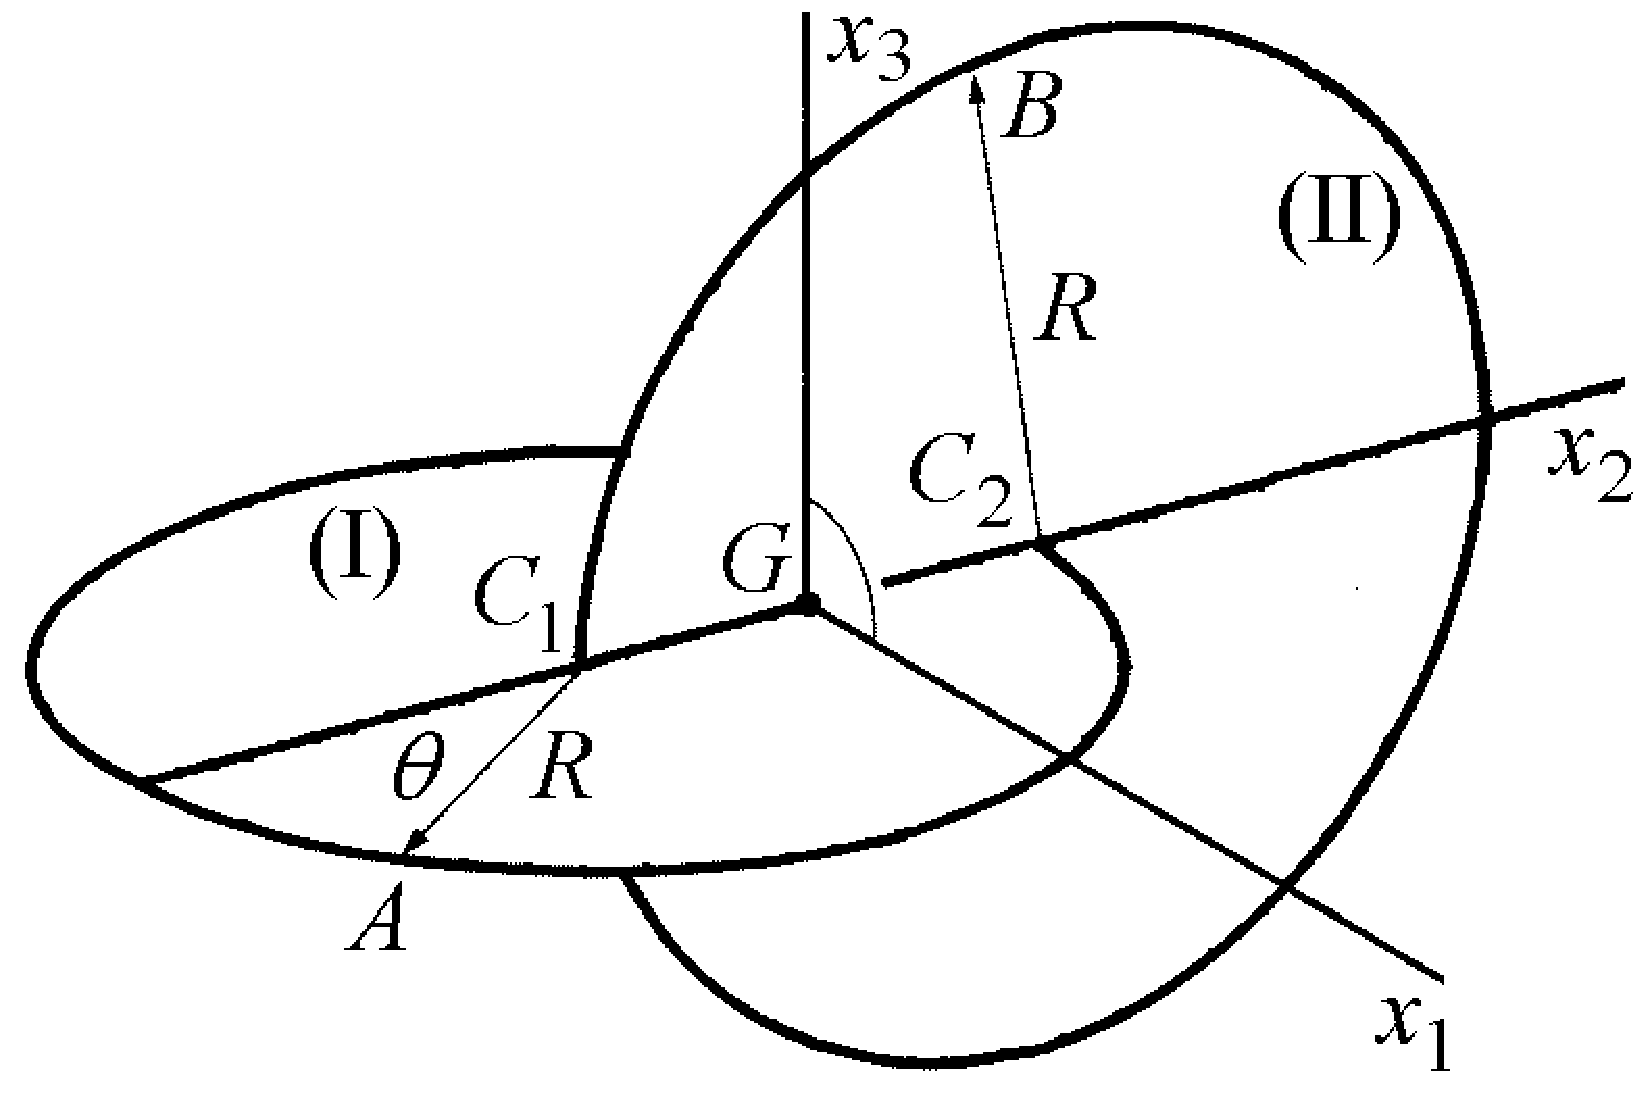
\includegraphics[height=4cm]{Oloid2}
\caption{The coordinate system $Gx_1x_2x_3$.}
\end{figure}




Let us consider the motion of the Oloid on a fixed horizontal plane. The Oloid is a developable surface comprises of two circles of radius $R$ whose planes of symmetry make a right angle between each other with the distance between the centers of the circles equals to their radius $R$. The resulting convex hull is called Oloid.

The Oloid have been constructed for the first time by Paul Schatz $[2$,$3]$. The geometric properties of the surface of the Oloid have been discussed in the paper $[1]$. The Oloid is also used for technical applications. Special mixing-machines are constructed using such bodies $[5]$. In our paper we make the complete kinematical analysis of motion of this object on the horizontal plane.

Further we briefly describe basic facts from Kinematics and Differential Geometry which we will use in our investigation.

\section*{Methods}

\subsection*{The Frenet - Serret formulas}
Consider a particle which moves along a continuous differentiable curve in three - dimensional Euclidean Space ${\cal R}^3$. We can introduce the following coordinate system: the origin of this system is in the moving particle, $\vec\tau$ is the unit vector tangent to the curve, pointing in the direction of motion, $\vec\nu$ is the derivative of $\vec\tau$ with respect to the arc-length parameter of the curve, divided by its length and $\vec\beta$ is the cross product of $\vec\tau$ and $\vec\nu$: $\vec\beta=\left[\vec\tau\times\vec\nu\right]$.

Then the Frenet - Serret formulas for the derivatives of $\vec\tau$, $\vec\nu$ and $\vec\beta$ are valid:
$$
\displaystyle\frac{d\vec\tau}{dt}=k\dot{s}\vec\nu,\quad
\displaystyle\frac{d\vec\nu}{dt}=-k\dot{s}\vec\tau+\ae\dot{s}\vec\beta, \quad
\displaystyle\frac{d\vec\beta}{dt}=-\ae\dot{s}\vec\nu.
$$

Here $d/dt$ is the derivative with respect to the time, $k$ is the curvature and $\ae$ is the torsion of the
curve. The tangent $\vec\tau$, the normal $\vec\nu$ and the binormal $\vec\beta$ unit vectors are known as the Frenet - Serret frame.

\subsection*{The Poisson formulas}

Let $\vec e_1$, $\vec e_2$, $\vec e_3$ is any moving coordinate system and let $\vec\omega$ be the angular velocity of this system. Then for the derivatives of $\vec e_1$, $\vec e_2$ and $\vec e_3$ the following Poisson formulas are valid:
$$
\frac{d\vec e_i}{dt}=\left[\vec\omega\times\vec e_i\right], \quad i=1,2,3.
$$

According to the Poisson formulas we can rewrite the Frenet - Serret formulas as follows:
$$
\frac{d\vec\tau}{dt}=\left[\vec\Omega\times\vec\tau\right],\quad
\frac{d\vec\nu}{dt}=\left[\vec\Omega\times\vec\nu\right],\quad
\frac{d\vec\beta}{dt}=\left[\vec\Omega\times\vec\beta\right],
$$
where $\vec\Omega=k\dot{s}\vec\beta+\ae\dot{s}\vec\tau$ is the angular velocity of the Frenet - Serret frame known also as the Darboux vector. In particular, for the plane curve we have $\ae=0$ and therefore
$$
\vec\Omega=k\dot{s}\vec\beta.\eqno(1)
$$

\subsection*{Two contact points}

Let us consider the rolling of the body consisting of two similar symmetric laminas in perpendicular planes connected to each other along the common axis of symmetry.This body rolls without slipping on the fixed horizontal plane. Let $G$ be the center of mass of the moving body and $K_1$, $K_2$ be two contact points of the body with the plane.

From the rolling conditions for the two contact points follows that the angular velocity is always parallel to the line between the contact points i.e.
$$
\left[\vec\omega\times\overrightarrow{K_1K_2}\right]=0.
$$

Now we introduce four coordinate systems. The first coordinate system is the fixed coordinate system $Oxyz$ with the origin at any point $O$ of the fixed plane. The $Oz$ - axis is directed upward. The second coordinate system is $Gx_1x_2x_3$ system with $Gx_2$ axis directed along the common axis of symmetry of the two laminas. The $Gx_3$ - axis  is perpendicular to the plane of the first lamina and the $Gx_1$ - axis is perpendicular to the plane of the second lamina. The third coordinate system is the Frenet - Serret frame $K_1\vec\tau\vec\nu\vec\beta$ for the bound of the first lamina: the $\vec\tau$ - vector is the tangent vector to the bound of the lamina, the $\vec\nu$ - vector is in the plane of the lamina and the $\vec\beta$ - vector coincides in the unit vector of $Gx_3$ axis (i.e. $\vec\beta$ is perpendicular to the plane of lamina). The fourth coordinate system is also the Frenet - Serret frame. The origin of this system is also in $K_1$, the first unit vector $\vec\tau_1$ of this system coincides with the vector $\vec\tau$ of the system $K_1\vec\tau\vec\nu\vec\beta$. The second vector $\vec\nu_1$ of this system is in the plane of motion and the third vector $\vec\beta_1$ is perpendicular to the plane of motion (i.e. the vector $\vec\beta_1$ coincides with the vector $\vec e_z$ of the system $Oxyz$). Therefore we can conclude that the coordinate system $K_1\vec\tau_1\vec\nu_1\vec\beta_1$ is the Frenet - Serret frame for the curve which is obtained by the motion of the contact point $K_1$ (i.e. it is a "trace" of the point of contact on the plane).

Let us try to find the angular velocity of the moving body. We will use the law of composition of angular velocities. Let us consider the systems $Oxyz$, $K_1\vec\tau\vec\nu\vec\beta$ and $Gx_1x_2x_3$. The absolute angular velocity of $Gx_1x_2x_3$ system with respect to $Oxuz$ system is the sum of angular velocity of $Gx_1x_2x_3$ with respect to $K_1\vec\tau\vec\nu\vec\beta$ and the angular velocity of $K_1\vec\tau\vec\nu\vec\beta$ with respect to $Oxyz$. But the angular velocity of $Gx_1x_2x_3$ system with respect to $K_1\vec\tau\vec\nu\vec\beta$ system can be found very easy: it is equal to $-k\dot{s}\vec\beta$. So we need calculate now the angular velocity of $K_1\vec\tau\vec\nu\vec\beta$ system with respect to $Oxyz$ system.

Let us denote by $\varphi$ the angle between two unit vectors $\vec\beta=\vec e_3$ and $\vec\beta_1=\vec e_z$. Then we can represent the angular velocity of $K_1\vec\tau\vec\nu\vec\beta$ system with respect to $Oxyz$ system is the sum of the angular velocity of $K_1\vec\tau\vec\nu\vec\beta$ system with respect to $K_1\vec\tau_1\vec\nu_1\vec\beta_1$ system and the angular velocity of $K_1\vec\tau_1\vec\nu_1\vec\beta_1$ system with respect to $Oxyz$ system. But the angular velocity of $K_1\vec\tau\vec\nu\vec\beta$ with respect to $K_1\vec\tau_1\vec\nu_1\vec\beta_1$ system is equal $\dot{\varphi}\vec\tau$ and the angular velocity of $K_1\vec\tau_1\vec\nu_1\vec\beta_1$ system with respect to $Oxyz$ system is equal $K\dot{s}\vec\beta_1$. Therefore finally we obtain:
$$
\vec\omega=\dot{\varphi}\vec\tau-k\dot{s}\vec\beta+K\dot{s}\vec\beta_1.
$$

Since $\vec\beta=-\vec\nu_1\sin\varphi+\vec\beta_1\cos\varphi$ we have
$$
\vec\omega=\dot{\varphi}\vec\tau_1+k\dot{s}\sin\varphi\vec\nu_1-k\dot{s}\cos\varphi\vec\beta_1+K\dot{s}\vec\beta_1.
$$

But from the rolling conditions we already obtained that the vector $\vec\omega$ is proportional to $\overrightarrow{K_1K_2}$ vector i.e. $\vec\omega$ is always in the plane of motion
$$
\vec\omega=\omega_1\vec\tau_1+\omega_2\vec\nu_1.
$$

This means that
$$
K=k\cos\varphi\quad\mbox{or}\quad \rho\cos\varphi=r,\eqno(2)
$$
where $\rho$ and $r$ are radii of curvature of the curve on the fixed plane (trajectory of the point $K_1$) and the bound of the first lamina.

\subsection*{Natural equations of a curve}

Let us consider the planar curve, defined by its parametric equations:
$$
{\vec r}={\vec r}\left(s\right)=x(s){\vec e_x}+y(s){\vec e_y},
$$
with the arc-length $s$ as a parameter. We denote by $\alpha (s)$ the angle between the unit tangent vector $\vec\tau$ to the given curve
$$
\vec\tau=\frac{d\vec r}{ds}=\frac{dx}{ds}{\vec e_x}+\frac{dy}{ds}{\vec e}_y
$$
and the unit vector $\vec e_x$ of the $Ox$ - axis. The initial value of $\alpha (s)$ at $s=0$ can be chosen within the value divisible by $2\pi$, for other points the angle $\alpha (s)$ is defined explicitly.

Since $\vec\tau (s)$ is the unit vector its projections on the $Ox$ and $Oy$ axes are $\cos\alpha$ and $\sin\alpha$ respectively. From the other side
$$
\vec\tau (s)=\cos\alpha\vec e_x+\sin\alpha\vec e_y=\frac{dx}{ds}\vec e_x+\frac{dy}{ds}\vec e_y,
$$
and therefore
$$
dx/ds=\cos\alpha,\quad dy/ds=\sin\alpha. \eqno(3)
$$

Moreover, using the first Frenet -- Serret formula we have
$$
\frac{d\vec\tau}{ds}=\left(-\sin\alpha\vec e_x+\cos\alpha\vec e_y\right)\frac{d\alpha}{ds}\vec\nu=k(s)\vec\nu,
$$
and hence
$$
d\alpha/ds=k(s).\eqno(4)
$$

This means that we can find the parametric equations of the curve if we know its curvature $k(s)$.

Thus we derived all the necessary facts for the investigation of the Oloid motion.

\subsection*{Coordinate frames and parametrization}

We consider now the motion of Oloid. Let two circles of the same radius $R$ in perpendicular planes be given such that each circle contains the center of the other. Then the convex hull of these circles is called Oloid. Let $k_A$ and $k_B$ be two circles of the same radius $R$ in perpendicular planes $\Pi_1$ and $\Pi_2$ such that $k_A$ passes through the center $M_B$ of $k_B$ and $k_B$ passes through the center $M_A$ of $k_A$ (Fig.~2).

According to the previous theory let us introduce the moving coordinate system $Gx_1x_2x_3$. The origin of this system will be at the midpoint $G$ of $M_AM_B$ (i.e. $G$ is the center of mass of the system). The $Gx_3$ - axis is perpendicular to the plane $\Pi_1$ of the first circle, $Gx_1$ - axis is perpendicular to the plane $\Pi_2$ of the second circle and $Gx_2$ axis is directed along the common axis of symmetry of two circles (Fig.~3).

We will parametrize the first circle by the angle $\theta$ between the negative direction of $Gx_2$ axis and the direction to the point of contact. Note that this parametrization is proportional to the arc-length parametrization $s$: $s=R\theta$. We introduce also the angle $\psi$ for the parametrization of the second circle: let $\psi$ be the angle between the positive direction of $Gx_2$ axis and the direction to the point of contact $B$. Then the radius - vector of the point $A$ can be written as follows:
$$
\overrightarrow{GA}=\vec r_1=R\sin\theta\vec e_1-\left(R/2+R\cos\theta\right)\vec e_2.
$$

The radius-vector of the point $B$ has the form:
$$
\overrightarrow{GB}=\vec r_2=\left(R/2+R\cos\psi\right)\vec e_2+R\sin\psi\vec e_3.
$$

When Oloid rolling on a fixed plane the three vectors $\vec r_1-\vec r_2$, $\vec r_1'$ and $\vec r_2'$ should be situated in this plane. We can write this condition as follows:
$$
\left|
\begin{array}{ccc}
R\sin\theta & -R-R\cos\theta-R\cos\psi & -R\sin\psi \\
R\cos\theta & R\sin\theta & 0 \\
0 & -R\sin\psi & R\cos\psi
\end{array}
\right|=0.
$$

As a result we have the following constraint between two parametrizations:
$$
\cos\psi+\cos\theta\cos\psi+\cos\theta=0.
$$

and now can obtain the radius -- vector $\overrightarrow{GB}=\vec r_2$ in the $\theta$ -- parametrization:
$$
\overrightarrow{GB}=\vec r_2=\left(\frac{R}{2}-\frac{R\cos\theta}{1+\cos\theta}\right)\vec e_2-\frac{R\sqrt{1+2\cos\theta}}{1+\cos\theta}\vec e_3.\eqno(4)
$$

Note here the interesting fact: the length of the vector $\overrightarrow{AB}$
$$
\overrightarrow{AB}=\overrightarrow{GB}-\overrightarrow{GA}=-R\sin\theta\vec e_1+\left(R+\frac{R\cos^2\theta}{1+\cos\theta}\right)\vec e_2-\frac{R\sqrt{1+2\cos\theta}}{1+\cos\theta}\vec e_3
$$
will be a constant
$$
AB=R\sqrt{3}.
$$

This feature is used in construction of Oloid.
The expression $(4)$ for the vector $\vec r_2$ then should give:
$$
0\leq 1+2\cos\theta \quad \forall \ \theta,\psi \in [-\frac{2\pi}{3},\frac{2\pi}{3}]
$$

\section*{Results}
\subsection*{Trajectories of the points of contact}

Let us derive now equation of the fixed plane in the $Gx_1x_2x_3$ coordinate system. We will write this equation in the form:
$$
LX+MY+NZ+P=0.
$$

Indeed points $A$, $B$ and the tangent vector to the first circle at $A$ are always in this plane therefore the following condition are valid:
$$
\left|
\begin{array}{ccc}
X-R\sin\theta & Y+\displaystyle\frac{R}{2}+R\cos\theta & Z \\
-R\sin\theta & R\left(1+\displaystyle\frac{\cos^2\theta}{1+\cos\theta}\right) & -\displaystyle\frac{R\sqrt{1+2\cos\theta}}{1+\cos\theta}\\
R\cos\theta & R\sin\theta & 0
\end{array}
\right|=0.
$$

From this condition after some simplifications we have the following expression for the plane of motion
$$
-\sin\theta X+\cos\theta Y+\sqrt{1+2\cos\theta}Z+\frac{R}{2}\left(2+\cos\theta\right)=0.
$$

The unit vector
$$
\vec n =-\sin\frac{\theta}{2}\vec e_1+\left(\frac{1}{2\cos\frac{\theta}{2}}-\cos\frac{\theta}{2}\right)\vec e_2+\frac{\sqrt{1+2\cos\theta}}{2\cos\frac{\theta}{2}}\vec e_3.
$$
is the normal vector to this plane. Therefore the angle between the plane of the first circle and the fixed plane is defined as follows:
$$
\cos\varphi=\left(\vec n\cdot\vec e_3\right)=\frac{\sqrt{1+2\cos\theta}}{2\cos\frac{\theta}{2}}.
$$

The radius of curvature of a circle at any point is equal to $R$. Thus using $(2)$ we can calculate the radius of curvature of a curve drawn by the point of contact $A$ on the fixed plane:
$$
\rho=\frac{R}{\cos\varphi}=\frac{2R\cos\frac{\theta}{2}}{\sqrt{1+2\cos\theta}}\quad\mbox{and}\quad
K=\frac{1}{\rho}=\frac{\sqrt{1+2\cos\theta}}{2R\cos\frac{\theta}{2}}.
$$

Having the expression for $K$ we can find the parametric equations of the trajectory of the point $A$ on the fixed plane.

For this purpose let us introduce the fixed coordinate system $Oxyz$. The origin $O$ of this system coincides with the point of contact of the first circle with the plane at $\theta=0$. The $Ox$ - axis is tangent to the first circle, the $Oz$ - axis is directed upwards. The $Oy$ - axis forms the right triple with the $Ox$ and $Oz$ axes. Then we get:
$$
\frac{d\alpha}{ds}=\frac{d\alpha}{Rd\theta}=K\left(\theta\right),\quad\mbox{i.e.}\quad \frac{d\alpha}{d\theta}=\frac{\sqrt{1+2\cos\theta}}{2\cos\frac{\theta}{2}}.
$$

Integration of this equation gives us the following expression for $\alpha$:
$$
\alpha=2\arctan\left(\frac{\sqrt{2}\sin\theta}{\sqrt{\left(1+\cos\theta\right)\left(1+2\cos\theta\right)}}\right)+
\arcsin\left(\frac{\left(\cos\theta-1\right)}{\sqrt{3}\sin\theta}\right).
$$

Using the trigonometric transformations and properties of the inverse trigonometric functions arctan and arcsin we reduce the expression for $\alpha$ to the form:
$$
\alpha=2\arcsin\left(\frac{2}{\sqrt{3}}\sin\frac{\theta}{2}\right)-\arcsin\left(\frac{\sin\frac{\theta}{2}}
{\sqrt{3}\cos\frac{\theta}{2}}\right).
$$

Then
$$
\sin\alpha=\frac{\sqrt{3}\sin\frac{\theta}{2}}{9\cos\frac{\theta}{2}}\left(5+4\cos\theta\right),\quad
\cos\alpha=\frac{\sqrt{3}}{9}\frac{\left(1+2\cos\theta\right)^{\frac{3}{2}}}
{\cos\frac{\theta}{2}}.
$$

Using these formulas together with $(3)$, $(4)$ we find after some trigonometric simplifications
$$
x_A\left(\theta\right)\!=\!\frac{2R\sqrt{3}}{9}\left(\arcsin\left(\frac{2}{\sqrt{3}}\sin\frac{\theta}{2}\right)\!+\!
\arcsin\left(\frac{\sin\frac{\theta}{2}}{\sqrt{3}\cos\frac{\theta}{2}}\right)\!+\!
2\sin\frac{\theta}{2}\sqrt{1\!+\!2\cos\theta}\right),
$$
$$
y_A\left(\theta\right)=\frac{8R\sqrt{3}}{9}\sin^2\left(\frac{\theta}{2}\right)-\frac{2R\sqrt{3}}{9}\ln\left(\cos\left(\frac{\theta}{2}\right)\right),
\quad -\frac{2\pi}{3}<\theta<\frac{2\pi}{3}.
$$

These equations give the parametric representation for the trajectory of the point $A$ on the fixed plane.

We can use the similar ideas in finding  the trajectory of point $B$, 
represented in the scalar form as:
$$
x_B\left(\theta\right)=x_A\left(\theta\right)+R\sqrt{3}\cos\left(\alpha+\gamma\right),\quad
y_B\left(\theta\right)=y_A\left(\theta\right)+R\sqrt{3}\sin\left(\alpha+\gamma\right).
$$

Here $\gamma$ is the angle between the vector $\vec e_{AB}$ and the tangent vector $\vec\tau$ to the first circle at $A$. The tangent vector $\vec\tau$ has the form:
$$
\vec\tau=\cos\theta\vec e_1+\sin\theta\vec e_2
$$
and therefore its scalar product with $\overrightarrow{AB}$ leads to:
$$
\left(\overrightarrow{AB}\cdot\vec\tau\right)=AB\left(\vec e_{AB}\cdot\vec\tau\right)=AB\cos\gamma=
R\sqrt{3}\cos\gamma=\frac{R\sin\frac{\theta}{2}}{\cos\frac{\theta}{2}},
$$
$$
\cos\gamma=\frac{\sin\frac{\theta}{2}}{\sqrt{3}\cos\frac{\theta}{2}},\quad
\sin\gamma=\frac{\sqrt{1+2\cos\theta}}{\sqrt{3}\cos\frac{\theta}{2}}.
$$

Further it is easy to find
$$
\sin\left(\alpha+\gamma\right)=\frac{7}{9}+\frac{4\cos^2\theta}{9\left(1+\cos\theta\right)},\quad
\cos\left(\alpha+\gamma\right)=-\frac{4\left(2+\cos\theta\right)\sin\frac{\theta}{2}}{9\left(1+\cos\theta\right)}
\sqrt{1+2\cos\theta}.
$$

Finally in the explicit form we have the following expressions for $x_B$ and $y_B$:
$$
x_B\left(\theta\right)\!=\!\frac{2R\sqrt{3}}{9}\left(\arcsin\left(\frac{2}{\sqrt{3}}\sin\frac{\theta}{2}\right)\!+\!
\arcsin\left(\frac{\sin\frac{\theta}{2}}{\sqrt{3}\cos\frac{\theta}{2}}\right)\!-\!
\frac{2\sin\frac{\theta}{2}}{\left(1\!+\!\cos\theta\right)}\sqrt{1\!+\!2\cos\theta}\right),
$$
$$
y_B\left(\theta\right)=\frac{7R\sqrt{3}}{9}+\frac{2R\sqrt{3}}{9\cos^2\left(\frac{\theta}{2}\right)}-\frac{2R\sqrt{3}}{9}\ln\left(\cos\left(\frac{\theta}{2}\right)\right),
\quad -\frac{2\pi}{3}<\theta<\frac{2\pi}{3}.
$$

\begin{figure}[h]
\centering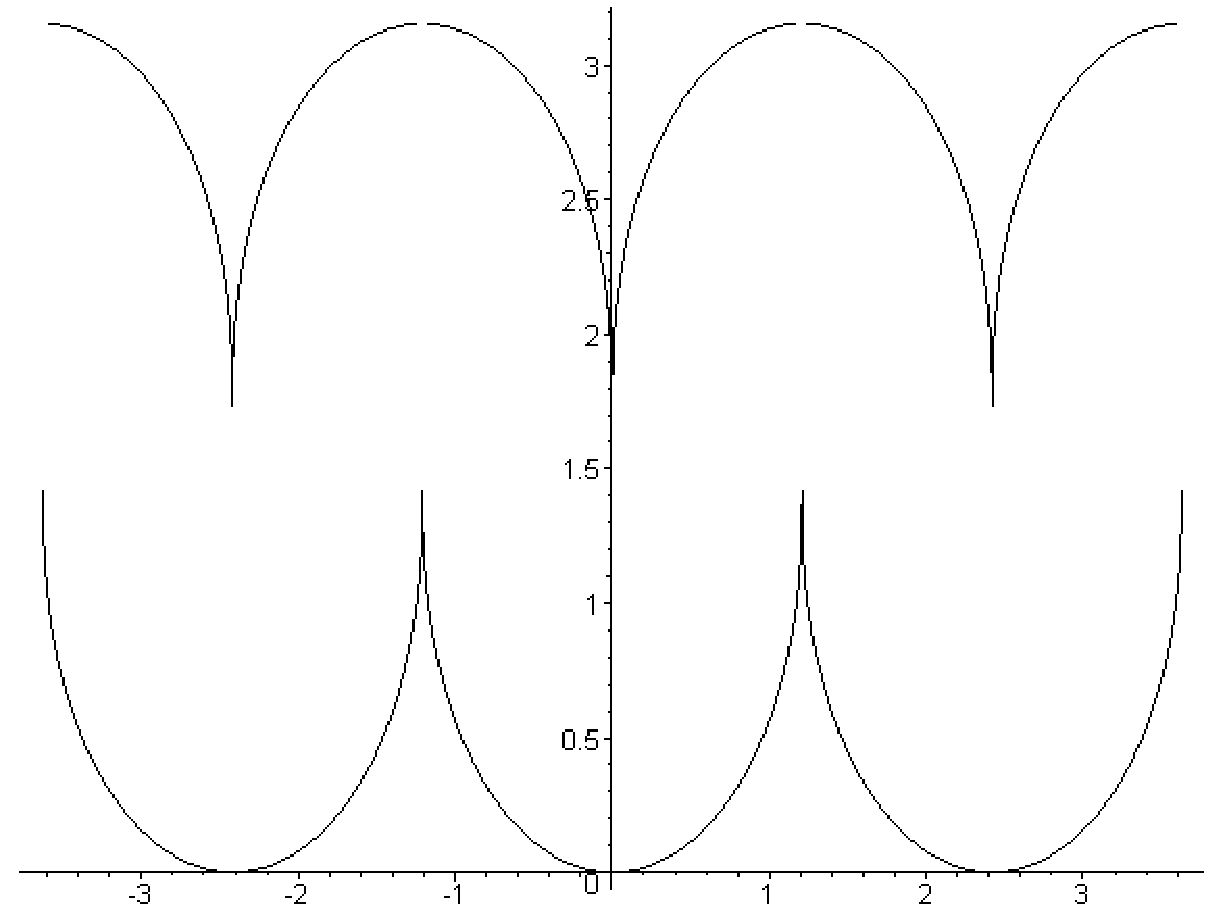
\includegraphics[height=6cm]{Oloid3}
\caption{Trajectories of points $A$ (bottom curve) and $B$ (upper curve) on the supporting plane.}
\end{figure}

These equations give the parametric representation for the trajectory of the point $B$ on the fixed plane. Figure 4 shows both trajectories on the fixed plane $Oxy$.

\subsection{Non-Obvious Dynamic Behaviors}
An unusual behavior was observed when simulation the dynamic motion of the oloid; we found that in simulation the waveform of the generalized speed changed qualitatively with different initial speeds.  The \ref{waveform} below demonstrates this. 
\begin{figure}[h!]
  \label{waveform}
  \centering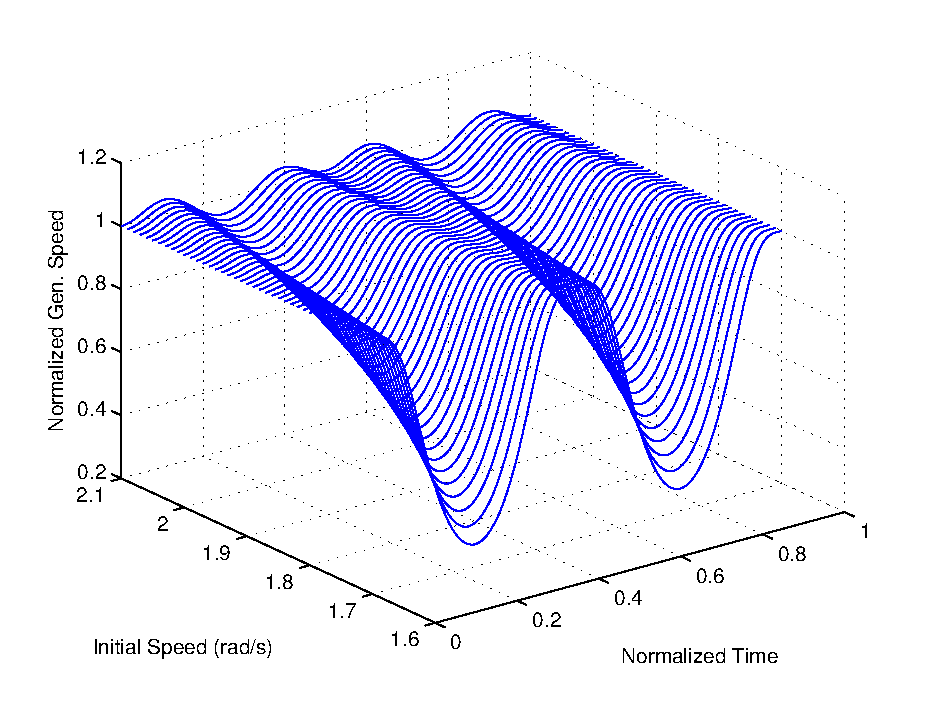
\includegraphics[height=10cm]{Waveform}
\caption{Qualitative Analysis of Generalized Speed Waveform (R = .1, G=9.8)}
\end{figure}
The speeds and times were normalized to the initial values and one cycle of the output.  It can be seen at the lower initial speeds that the speed starts by falling and at the higher initial speeds it starts by rising.  We believe this behavior to be unusual for such a simple, deterministic, one degree of freedom system.  Also visible is the change in shape of waveform throughout the cycle from two large speed minimums to four smaller speed minimums.   


\section{Conclusions}
We investigate here the motion of the Oloid toy on the fixed horizontal plane. Parametric equations for the trajectories of points of contact of the Oloid with the plane are derived.


\begin{thebibliography}{99}
\bibitem{Development} Dirnb\"ok H., Stachel H. (1997) The Development of the Oloid.  {\em J. Geometry Graphics}
{\bf 1}:105-118.
\bibitem{Schatz1} Schatz P. (1975) Rhythmusforschung und Technik. Verlag Freies Geistesleben, Stuttgart.
\bibitem{Schatz2} Schatz P. (1933) Deutsches Reichspatent Nr. 589 452 in der allgemeinen Getriebeklasse.
\bibitem{Spong} Spong M., Hutchinson S. and Vidyasagar M. (2005) Robot Modeling and Control. Wiley and Sons.
\bibitem{Bio} Bioengineering AG (Sagenrainsrt. 7, 8636 Wald, Switzerland).
\end{thebibliography}

\end{document}
